\pagestyle{fancy}
\chapter{Servidores remotos y clientes. Web Mapping}
\label{Servidores_y_clientes_remotos}

\chapterauthor{Olaya, Víctor; Turton, Ian; Fonts, Oscar}

\bigskip

\begin{intro}
El avance de las redes locales y de Internet ha permitido que se acceda a la información geográfica contenida en un SIG utilizando el paradigma cliente--servidor. Para ello es necesario contar con componentes en el lado servidor que distribuyan la información y componentes en el lado del cliente para acceder a esta. En este capítulo veremos las características de ambos elementos y cómo estos responden a las necesidades que el trabajo con datos remotos plantea en el ámbito SIG. Enfocaremos particularmente el capítulo a las tecnologías de \emph{Web Mapping}, las cuales permiten incorporar las ideas de los SIG dentro de paginas Web, utilizando un navegador Web como aplicación principal. \index{Web Mapping}
\end{intro}

\section{Introducción}

Del mismo modo que podemos acceder a otros tipos de información a través de Internet o de una red local, también podemos emplear esta para acceder a información geográfica y trabajar con ella dentro de un SIG. En el contexto actual, no puede dependerse en un SIG únicamente de datos locales en forma de archivos en el mismo ordenador en el que se trabaja, sino que es necesario poder operar con datos remotos. Las redes son la vía para la difusión de todo tipo de información, entre ella la información geográfica.

Los datos espaciales pueden ofrecerse a través de una red de la misma manera que se ofrecen otro tipo de datos como imágenes o texto en una pagina Web. Para que en este proceso se maximicen las posibilidades que esos datos ofrecen, es necesario disponer de tecnologías adaptadas basadas en las tecnologías fundamentales de las redes, pero particularizadas al tipo de datos concreto que se maneja y los posibles usos que pueden darse.

Estas tecnologías son variadas y, como cabe esperar, han evolucionado paralelamente a otras basadas en la Web, añadiendo progresivamente elementos tales como una mayor interactividad o flexibilidad Web. Las páginas estáticas que formaban Internet hace unos años, muy limitadas en cuanto a sus posibilidades, han dado paso a lo que hoy se conoce como Web 2.0, donde encontramos \emph{blogs}, \emph{wikis} y otros tipos de páginas Web con capacidades mucho mayores y que permiten al usuario un trabajo muy distinto.\index{Interactividad}

Una evolución similar han seguido las aplicaciones de la Web relacionadas con la información geográfica, habiendo ganado día tras día en riqueza hasta el estado actual donde pueden llegar a ofrecer casi tantas funcionalidades como un SIG de escritorio. Los mapas estáticos que constituían los primeros elementos con componente geográfica en la Web han evolucionado hasta verdaderas aplicaciones que pueden convertir un navegador Web en una plataforma SIG completa. En su avance, las tecnologías Web van tomando elementos que ya conocemos de los SIG de escritorio, con objeto de trasladar toda su potencia al entorno de Internet, y uniéndola así con las capacidades que la red tiene como espacio común de actividad y conocimiento.

Aunque el objetivo final sea trasladar los SIG de escritorio a la red, las tecnologías necesarias distan bastante de las tecnologías SIG en sentido clásico, de la misma forma que, aun trabajando con un tipo de datos similar, un procesador de textos se diferencia mucho de un navegador Web. 

Fundamentalmente, estas tecnologías Web han de responder a dos necesidades principales: servir un elemento a través de la red y tomar este para emplearlo. Es decir, tomar y recibir el elemento que es objeto de interés. Distinguimos así los conceptos de \emph{servidor} y \emph{cliente}, que debemos ver con algo más detalle antes de continuar.\index{Servidor}\index{Cliente}

\section{¿Cómo funciona Internet?}

Estamos acostumbrados a utilizar Internet a través de aplicaciones tales como navegadores Web, y en muchos casos desconocemos cómo se realiza ese proceso tan cotidiano hoy en día. Los fundamentos que residen detrás de la consulta de una simple página Web son esencialmente los mismos que vamos a encontrar para el caso de las tecnologías SIG en la red, por lo que es necesario conocerlos al menos someramente para poder entender el proceso que tiene lugar cuando empleamos una tecnología SIG en Internet.

Cuando consultamos una página Web existen tres elementos fundamentales que entran en juego: la propia red que hace de nexo entre sus elementos, nuestro ordenador que es el que realiza la petición de consulta, y la máquina donde se encuentra almacenada esa página que queremos consultar.

Conocemos como \emph{servidor} al elemento encargado de \emph{servir} algún tipo de contenido. En el ámbito SIG, se trata fundamentalmente (aunque no con carácter exclusivo) de datos geográficos, que constituyen el principal producto que se distribuye a través de la red dentro de nuestro campo. En el ejemplo anterior, la máquina que contiene la página de interés es el servidor. También se conoce como servidor el programa que, residiendo en esa máquina, interpreta la petición y la procesa, sirviendo así la página.

El \emph{cliente} es responsable de \emph{pedir} ese dato al servidor, tomarlo y trabajar con él. Nuestro navegador Web es el cliente en este caso, ya que es el que realiza la petición. Para ello, basta con introducir la dirección Web\footnote{Técnicamente, una dirección Web como esta se conoce como URL (Uniform Resource Locator)} correspondiente en la barra de direcciones del navegador. Al hacer esto, proporcionamos una serie de datos que son los que se emplean para realizar el proceso, y que vamos a ver a continuación en detalle.\index{URL}

Supongamos la dirección Web \texttt{http://volaya.es/writing}, en la cual puedes encontrar información relacionada con este libro e incluso descargarlo. Si visitas esa página estás efectuando una petición a través de esa URL, la cual se compone de las siguientes partes:

\begin{itemize}
	\item \texttt{http}: El protocolo a usar, que define la forma en que se van a comunicar cliente y servidor. Aunque este es el más habitual, existen muchos otros tales como \texttt{ftp} o \texttt{mailto}. Puede encontrarse más acerca de estos protocolos en \cite{protocolosWeb}.
	\item \texttt{volaya.es}: Esta cadena identifica la máquina donde reside la página que buscamos. Es en realidad una versión más legible para el ojo humano de un código numérico que indica la dirección concreta. El navegador lo convierte en realidad en algo como 128.118.54.228.
	\item \texttt{writing}: La página que buscamos dentro de todas las que hay en esa máquina. Se expresa como una ruta a partir del directorio raíz del servidor, que no es necesariamente el directorio raíz de la maquina servidora.
\end{itemize}
\index{FTP}

El proceso mediante el que podemos ver esa página en un navegador Web comprende los cuatro pasos siguientes:

\begin{enumerate}
	\item El cliente realiza la petición.
	\item La petición se conduce a través de la red hasta el servidor.
	\item El servidor busca la página y la devuelve a través de la red en caso de encontrarla, o devuelve una pagina de error en caso de no tenerla.
	\item El cliente recibe la página y la representa.
\end{enumerate}


La figura \ref{Fig:Asi_funciona_internet} muestra un esquema de este proceso.

\begin{figure}[!hbt]   
\centering
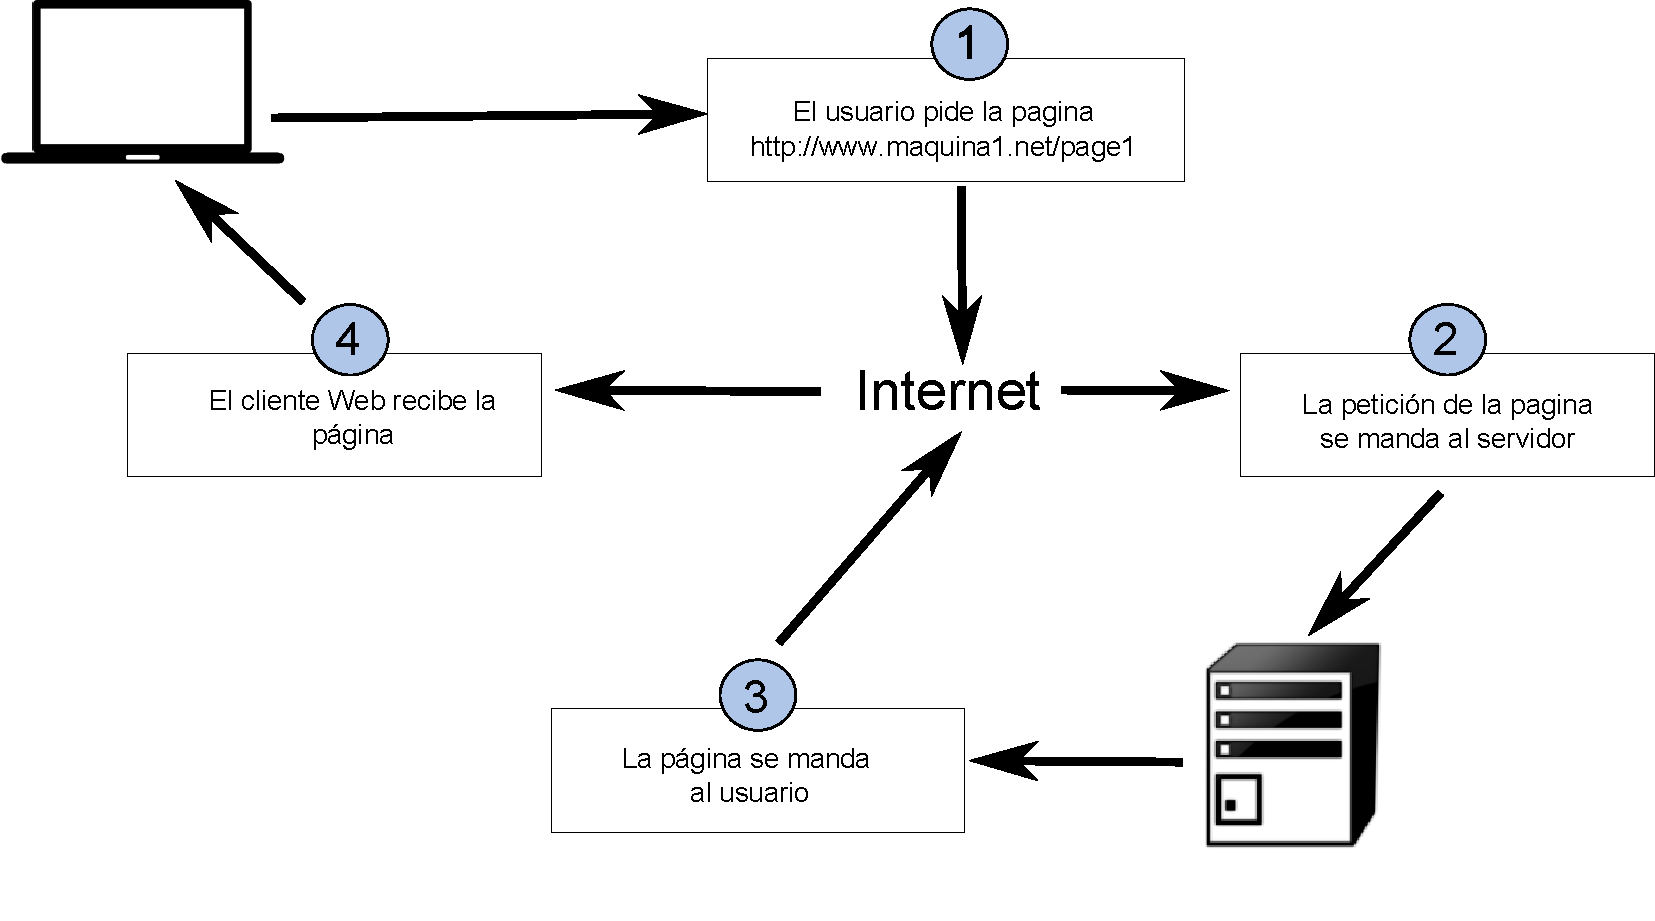
\includegraphics[width=.95\mycolumnwidth]{Cliente_servidor/Asi_funciona_internet.pdf}
\caption{\small Esquema del proceso de consulta de una página Web desde un navegador.}
\label{Fig:Asi_funciona_internet} 
\end{figure}

\section{El valor de las tecnologías SIG Web}

Antes de abordar la parte más técnica de las tecnologías Web SIG, veamos el significado de estas y la función que cumplen. Entenderemos en este contexto como tecnologías Web SIG a todos aquellos elementos que permiten la representación de cartografía como un contenido más de una página Web. Esto es lo que se engloba bajo la denominación genérica de \emph{Web Mapping}.

Aunque este capítulo está dedicado a las tecnologías Web dentro del ámbito SIG, y estas incluyen tanto servidores como clientes, las formas en las que se presentan los elementos del \emph{Web Mapping} dependen fundamentalmente del cliente, el cual es en general un simple navegador. 

Como vimos en el capítulo dedicado a los SIG de escritorio, estos pueden acceder a datos remotos, y para ello necesitan realizar una petición a un servidor siguiendo el esquema que hemos visto en el apartado anterior. Una vez que los datos están en el SIG (es decir, el servidor ha devuelto a este los datos que había pedido), podemos operar con ellos usando las herramientas que ya conocemos.

En un entorno Web \emph{sensu stricto} tal como el de un navegador, las posibilidades son, no obstante, distintas, pues se trata de combinar los elementos cartográficos con los restantes elementos que forman parte habitual de una página Web. Las tecnologías Web de corte SIG se han desarrollado principalmente para su trabajo dentro de un navegador, es decir, como una alternativa a los SIG de escritorio o para alcanzar áreas nuevas en el trabajo con información geográfica digital. Su incorporación en los SIG de escritorio aumenta las capacidades de estos, pero la principal potencia de estas tecnologías surge cuando se unen a otras funcionalidades de tipo Web.

En resumen, el objetivo básico que pretenden cumplir las tecnologías que vamos a ver, especialmente las del lado del cliente, es llevar las funcionalidades de un SIG a la Web, para así compartir la potencia de ambos componentes.  Las ventajas de llevar el SIG a la Web en lugar de incorporar los elementos de esta última en un SIG de escritorio tradicional son notables, y existen grandes diferencias entre las soluciones que se obtienen en ambos casos. Estas diferencias tienen que ver sobre todo con los usuarios y su perfil, así como con el diseño mismo de las aplicaciones. 

Mientras que un SIG de escritorio se orienta principalmente a usuarios más especializados, poder dotar a un sencillo navegador Web de capacidades de visualización o edición de información geográfica hace que estos lleguen a un público distinto y abre nuevas posibilidades. Los usuarios avanzados encuentran igualmente utilidad en el \emph{Web Mapping}, que se complementa en muchos terrenos con los SIG de escritorio. Por su parte, los usuarios no especializados, desconocedores de otras tecnologías SIG, pueden incorporarse al ámbito SIG a través de las tecnologías Web.

Algunas de las ideas fundamentales que caracterizan a las tecnologías de \emph{Web Mapping} y su papel actual son las siguientes:

\begin{itemize}
	\item \textbf{No es necesario un software SIG específico}. Al menos, no es necesario desde el punto de vista del usuario, que no ha de instalar nada adicional en su ordenador. Acceder a cartografía remota e incluso a funcionalidades avanzadas basadas en esos datos no requiere más que un simple navegador Web, algo presente en cualquier ordenador hoy en día. La barrera que puede suponer el trabajar con una aplicación específica se diluye cuando incorporamos las capacidades de esta en algo tan habitual como un navegador.
	\item \textbf{Perfil menos técnico}. No solo las aplicaciones están pensadas para su utilización por parte de usuarios no especializados, sino que la incorporación de estos al ámbito SIG hace que la cartografía deje de ser un elemento propio de esos usuarios más técnicos. Poniendo al alcance de todos las capacidades de edición y creación de cartografía hace que cualquiera pueda generar su propia información geográfica no especializada y además ponerla a disposición de otros usuarios.
	\item \textbf{Potenciamiento del trabajo colaborativo}. La red es un punto de encuentro que favorece de forma natural la colaboración. Proyectos como la Wikipedia, posibles gracias a esta capacidad de  Internet para facilitar el trabajo común de múltiples personas, tiene sus equivalentes en el ámbito de la información geográfica. Los SIG dejan de ser algo personal reducido al ámbito de un ordenador o una pequeña red, para ser algo global en una red de muchos SIG interconectados. Y más importante que esto, los datos también se hacen globales, pudiendo ser empleados e incluso editados por todos.
	\item \textbf{Información más actualizada}, incluso en tiempo real. La Web es el canal ideal para transmitir la información de forma inmediata y flexible. A las ventajas de los datos digitales sobre los analógicos en este sentido, que ya vimos en el capítulo \ref{Introduccion_datos}, hay que sumar que la sencillez de acceso que aporta una interfaz Web hace todavía más accesible la información geográfica más reciente.
	\item \textbf{Independencia del sistema}. Un mapa Web puede verse y usarse del mismo modo en cualquier ordenador, con independencia del sistema operativo, el navegador e incluso el dispositivo empleado (PC, PDA, etc.). Si este mapa se basa en estándares abiertos, la solución es todavía más interoperable, como veremos en el capítulo \ref{Estandares}.\index{Estándares}\index{PDA}
	\item \textbf{Personalización de aplicaciones}. Una de las tendencias más importantes en el ámbito del \emph{Web Mapping} es la creación de aplicaciones que personalizan una base común para un determinado uso. Sobre una base compuesta por un juego de datos genérico (generalmente imágenes de satélite y mapas base tales como un mapa de carreteras) y una aplicación SIG, se crean pequeñas aplicaciones de forma sencilla, a las cuales se pueden añadir de modo también simple nuevos datos. Estas aplicaciones se conocen como \emph{mashups}, y una vez creadas puede incorporarse a una página Web distinta. Dedicaremos una sección completa de este capítulo a desarrollarlas en detalle.\index{Mashup}
	
	Mediante uno de tales \emph{mashups}, un usuario puede crear, sin excesivos conocimientos sobre SIG, una aplicación particular que ponga sobre ese juego de datos general los emplazamientos de, por ejemplo, todos aquellos que visitan su página Web. Las posibilidades en este sentido son prácticamente infinitas, y proliferan de forma exponencial en Internet.
	\item \textbf{Combinación de cartografía y otros elementos}. Si llevamos las capacidades SIG a un navegador, además de estas dispondremos en ese navegador de muchas otras posibilidades, tales como la representación de elementos multimedia (vídeo, sonido, etc.) o el uso de hiperenlaces. El navegador es hoy en día la aplicación versátil por excelencia, y ello hace que podamos añadir a las capacidades SIG una larga serie de otras funcionalidades no relacionadas directamente con la información geográfica, y no presentes en su mayoría en los SIG de escritorio.
\end{itemize}

La importancia de las tecnologías Web se debe, por tanto, principalmente a un razón social y no a una tecnológica, aunque es innegable que las tecnologías novedosas que se desarrollan en este campo aportan al ámbito SIG posibilidades antes desconocidas. Estas nuevas posibilidades enriquecen notablemente los SIG de escritorio si estos implementan las capacidades de acceso a datos remotos, ampliando el alcance de ese tipo de aplicaciones. Cuando se implementan, sin embargo, en un entorno puramente Web tal como en el seno de un navegador y se crea una página Web con elementos SIG, se consigue ampliar el abanico de usuarios potenciales y así también crecen las posibilidades y las formas en que el propio SIG puede presentarse.


\section{Formas de cartografía en la Web}

Las formas en las que pueden presentarse las tecnologías SIG dentro de un entorno Web varían en cuanto a su similitud con los SIG de escritorio, incorporando más o menos elementos de los que son habituales en este tipo de aplicaciones. Como parece lógico pensar, ha existido una evolución progresiva, de tal modo que en la actualidad existen más elementos propios de los SIG de escritorio dentro de las tecnologías Web SIG, y la cartografía Web hoy en día permite realizar un trabajo más similar al que se desarrolla en un SIG clásico.

Una primera y sencilla clasificación de los tipos de cartografía Web es la que divide esta en mapas \emph{estáticos} y \emph{dinámicos}\cite{Kraak2001Francis}. 

Un mapa estático es simplemente una imagen con información cartográfica, la cual no permite ningún tipo adicional de trabajo con ella que no sea la mera observación. En este sentido, se asemeja a un mapa clásico, donde el usuario no puede interactuar directamente con el contenido del mapa. A efectos de trabajo real, las posibilidades son aún menores ya que acciones tales como mediciones tampoco pueden realizarse, ni siquiera con medios mecánicos como el caso de un mapa en papel. Junto a esto, la resolución de una pantalla común es mucho menor que la que presenta un mapa impreso, con lo que la calidad del mapa no es comparable.

Este tipo de mapas, por tanto, no responden a las funcionalidades que un SIG ha de tener para poder prestar utilidad en el manejo y uso de información geográfica, y difieren notablemente de un SIG de escritorio, incluso en la versión más básica y primitiva de estos últimos.

Incorporar este tipo de mapas a una página Web no requiere ninguna tecnología particular, y puede llevarse a cabo con elementos genéricos tanto del lado del cliente como del servidor, pues el dato realmente no es un dato geográfico como tal, sino una mera imagen (y esa imagen no va acompañada de información tal y como su sistema de referencia), algo para lo cual cualquier servidor o cliente actual ofrece soporte.

La figura \ref{Fig:XeroxPARC} muestra una imagen de una primigenia cartografía Web presentada a través del visor Xerox PARC Map Viewer\index{Xerox PARC Map Viewer}.

\begin{figure}[!hbt]   
\centering
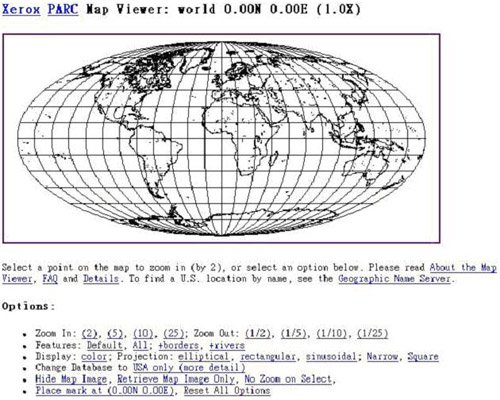
\includegraphics[width=.85\mycolumnwidth]{Cliente_servidor/XeroxPARC.png}
\caption{\small Visor de mapas Xerox PARC Map Viewer, uno de los primeros en su campo}
\label{Fig:XeroxPARC} 
\end{figure}


Por su parte, un mapa dinámico es aquel que no se compone de una imagen inmóvil, sino que esta varía y se adapta en función de los requerimientos del usuario o según alguna serie de parámetros prefijados. De acuerdo con esto, los mapas dinámicos pueden ser interactivos o no, dependiendo de si es el usuario quien directamente modifica la representación del mapa.

Como ejemplo de mapa dinámico no interactivo podemos citar mapas animados que encuadran una determinada zona y muestran la variación de una variable a lo largo del tiempo. Mapas de variables climatológicas o una serie animada de mapas que reflejan el avance de un incendio son ejemplos habituales de este grupo.

Tampoco en este tipo de mapas aparecen las funciones esperables en una aplicación SIG, y una vez más no se requieren tecnologías específicas para poder incorporar este tipo de elementos en una página Web.

La interactividad es la que aporta las posibilidades necesarias para comenzar a incorporar funciones SIG a la cartografía Web, y sin ella no podemos hablar en realidad de tecnologías SIG puramente dichas.

La forma de interactividad más básica que se implementa en una página Web en el trabajo con cartografía es la que permite la modificación de la forma en que los datos geográficos se visualizan. Las herramientas que permiten modificar la escala de visualización (acercarse o alejarse) y desplazar el mapa, las cuales ya nombramos como capacidades básicas en los SIG de escritorio, aportan a la cartografía Web muchas posibilidades nuevas. Entre ellas, es de destacar que mediante estas herramientas la extensión de los datos no se encuentra limitada por la propia extensión de la pantalla o la dimensión del navegador. 

Si se trabaja con imágenes estáticas, trabajar con datos que cubran toda la extensión del globo implica hacerlo a una escala de muy poco detalle, pues ha de representarse toda la imagen de forma simultanea. Permitiendo que el usuario elija la escala de representación y ajuste la extensión con la que se desea trabajar, un navegador Web se convierte en una ventana hacia datos que pueden tener cualquier extensión y volumen, y hacia el trabajo con ellos de forma dinámica e interactiva.

Esto es de especial importancia si pensamos que las máquinas que se encuentran al otro lado (en el servidor) son ordenadores potentes con gran capacidad, que pueden almacenar enormes juegos de datos. Un juego de datos con imágenes de todo el mundo a gran resolución ocupa un tamaño que probablemente lo haga inutilizable en un ordenador personal (además de que ese juego probablemente quede fuera del alcance del usuario de ese ordenador en lo que a su adquisición respecta), pero puede perfectamente ser servido desde un potente servidor, sirviendo en cada caso la <<porción>> de él que cada usuario requiere según utiliza el cliente correspondiente. En esto se basan gran parte de servicios y de aplicaciones desarrolladas sobre ellos, como veremos más adelante.

De especial importancia para el desarrollo de estas capacidades ha sido la popularización y mejora de las tecnologías que permiten el desarrollo de las denominadas \emph{Aplicaciones Ricas de Internet} (RIA)\footnote{Rich Internet Applications}. Este tipo de aplicaciones llevan a la Web algunos elementos de las tecnologías de escritorio, y en general permiten optimizar el volumen de datos necesario para operar con la aplicación dentro del entorno del navegador.\index{Rich Internet Applications (RIA)}

Si no se emplean estas tecnologías, un cambio mínimo en la configuración de la pagina por parte del usuario (por ejemplo, modificar el encuadre del mapa en una aplicación SIG), requiere la recarga total de la página, de la misma forma que sucede cuando hacemos clic en un hiperenlace. En realidad, estamos pasando a una página Web distinta. 

En un entorno RIA, sin embargo, se cargan al inicio (en el primer acceso a la página) los elementos que constituyen la aplicación en sí, y posteriormente se transmiten únicamente los datos que vayan siendo necesarios a medida que el usuario opere con la aplicación. Esto mejora notablemente la sensación del usuario, ya que este nunca tiene ante sí una pantalla sin contenido mientras se carga la página, puesto que esta ya no ha de cargarse de nuevo, y la carga de datos puede además realizarse mientras el propio usuario opera.

AJAX \footnote{Asynchronous JavaScript And XML} \cite{garrett2005ajax} es una técnica de desarrollo muy popular en este sentido, y de la que los SIG Web hacen uso habitualmente. La figura \ref{Fig:AJAX} muestra una comparación entre el esquema de una aplicación Web tradicional y una basada en AJAX. \index{AJAX}

\begin{figure}[!hbt]   
\centering
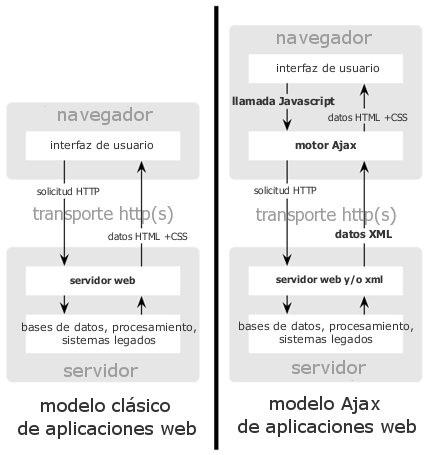
\includegraphics[width=.55\mycolumnwidth]{Cliente_servidor/ajax.png}
\caption{\small Comparación entre el esquema de una aplicación Web tradicional y una basada en AJAX.(adaptado de \cite{garrett2005ajax}).}
\label{Fig:AJAX} 
\end{figure}

Profundizar más en estos aspectos es, no obstante, demasiado técnico para el enfoque de este libro, no siendo necesario además para la comprensión de las tecnologías Web desde el punto de vista del usuario. Tan solo es necesario diferenciar entre el comportamiento de una página Web anterior a la introducción de estas técnicas, en la cual cualquier interacción (clic del ratón) suponía una recarga completa de la página, mientras que en el caso de una RIA, la experiencia es más fluida y cercana a la que se tiene usando una aplicación de escritorio.

\begin{figure}[!hbt]   
\centering
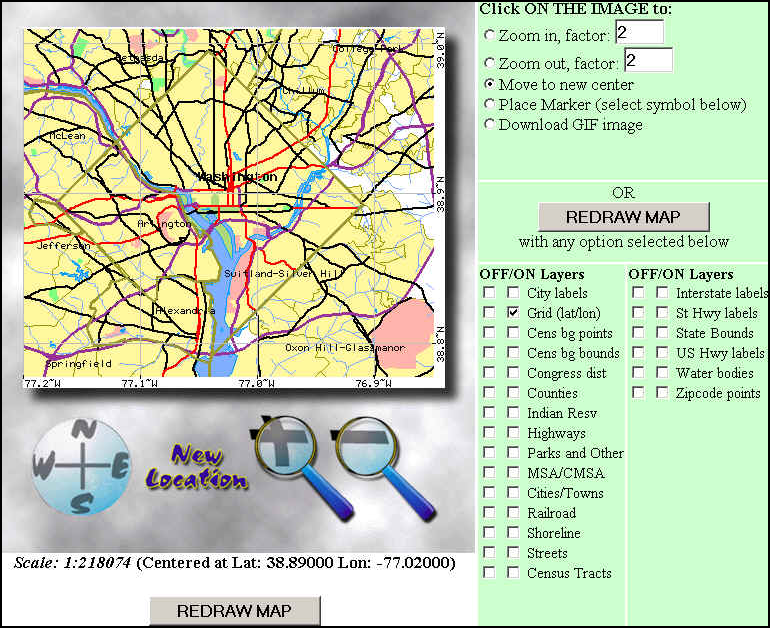
\includegraphics[width=.9\mycolumnwidth]{Cliente_servidor/tiger.png}
\caption{\small Interfaz de TIGER MapServer (año 1997)}
\label{Fig:Tiger} 
\end{figure}


La figura \ref{Fig:Tiger} muestra el aspecto de una aplicación de \emph{Web Mapping} previa a la introducción de tecnologías como AJAX, en particular la Web a través de la que se accedía a los datos del proyecto TIGER, creado por el U.S Census Bureau.\index{TIGER}\index{U.S. Census Bureau}


Además de modificar la zona representada, un usuario debe poder modificar la forma en que los datos dentro de esa zona se muestran. Es decir, debe poder cambiar el estilo de los elementos representados, variando colores o formas de la misma manera que esto puede hacerse en un SIG de escritorio. Asimismo, muchas aplicaciones Web permiten la consulta de varias capas de datos, incluso de datos provenientes de varios servidores distintos, datos que no necesariamente han de mostrarse todos simultáneamente. Igual que en un SIG de escritorio seleccionamos unas u otras capas para su visualización y podemos alterar el orden de representación de estas, también podemos realizar estas operaciones en una aplicación SIG Web.

Esto hace que una aplicación SIG dentro de un navegador se convierta en una herramienta completa para el acceso a uno o varios juegos de datos remotos cuyo contenido es abundante (no solo en extensión sino también en tipos de datos suministrados), ya que permite una gran configurabilidad y deja en manos del cliente (esto es, del usuario), la forma de tomar esos datos y mostrarlos.

Las capacidades de edición también tienen lugar en los SIG Web, ampliando las posibilidades que la interactividad más básica ofrece. Un usuario puede añadir su propia información a un SIG Web o bien modificar una capa existente empleando su navegador. Las tecnologías SIG siguen en este sentido a las tecnologías Web más generales, adoptando los conceptos de la Web 2.0 y ampliando las posibilidades de los usuarios de colaborar directamente en los contenidos de la red. Por ejemplo, \emph{OpenStreetMap} \cite{webOSM} es un sitio equivalente a la bien conocida Wikipedia, en el cual los usuarios pueden añadir sus propias descripciones de elementos geográficos que ellos mismos definen.\index{Wikipedia}\index{OpenStreetMap}

A estas mismas tecnologías se les puede dar usos más restringidos sin que necesariamente sea dentro de un proyecto colaborativo abierto. Por ejemplo, una administración local puede dar acceso a los propietarios de suelo para que puedan consultar su catastro, mediante un sistema de autenticación conveniente, incluso editar información de sus parcelas. Está información puede ser de tipo no espacial (es decir, los límites de las parcelas serían fijos), ya que las capacidades de edición no han de limitarse a la componente espacial.\index{Autenticación}

Por último, y aunque en la actualidad son pocos los servicios de este tipo que existen, y no pueden compararse las prestaciones con las que ofrecen los SIG de escritorio, la cartografía Web puede ofrecer herramientas de análisis. Además de representar un conjunto de datos geográficos y permitir al usuario navegar en ellos e incluso editarlos, pueden extraerse resultados a partir de esos datos. 

Un tipo de aplicación bastante extendida de este tipo es el cálculo de rutas óptimas. A partir de una capa con vías de comunicación un usuario establece un punto de salida y otro de destino y la aplicación Web calcula la ruta que optimiza el tiempo empleado o la distancia total recorrida, según lo explicado en el capítulo \ref{Costes}. \cite{webGuiaCampsa} es un ejemplo de este tipo de aplicaciones en el cual la interfaz no es la de un SIG de escritorio habitual, sino que se introducen los lugares de origen y destino tecleando sus nombres y después la ruta calculada se muestra sobre un mapa y también como un conjunto de indicaciones a seguir. Es decir, que sobre una base de cálculo SIG se crea una aplicación más completa que la que es habitual encontrar en un SIG, aprovechando la mayor riqueza de elementos que pueden utilizarse dentro de un navegador Web.

El término \emph{Web Mapping}, habitualmente empleado para designar a la cartografía Web, se sustituye por \emph{Web GIS} a medida que las capacidades de las aplicaciones Web aumentan, para indicar así que todos los componentes que forman parte de un SIG en su sentido clásico, esto es, un SIG de escritorio, se incorporan a dicha aplicación Web.\index{Web GIS}

La figura \ref{Fig:Tipos_Cartografia_Web} muestra un esquema de la evolución de la cartografía Web a través de los tipos anteriormente descritos.

\begin{figure}[!hbt]   
\centering
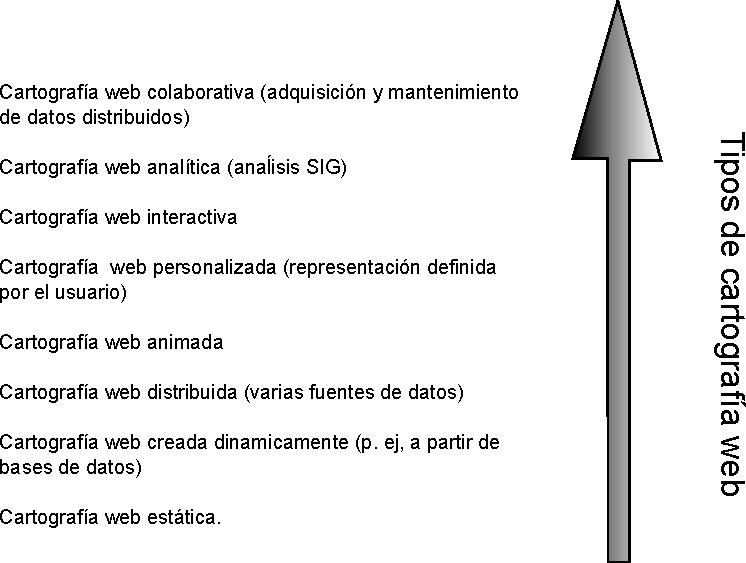
\includegraphics[width=.6\mycolumnwidth]{Cliente_servidor/tipos_cartografia_web.pdf}
\caption{\small Evolución de los tipos de cartografía en la Web (según \cite{Kraak2001Francis})}
\label{Fig:Tipos_Cartografia_Web} 
\end{figure}

\subsection{ \emph{Mashups}}

Se conoce como \emph{mashup} o \emph{aplicación Web híbrida} a una aplicación que basa sus contenidos en los de otras páginas Web, integrándolos y creando una nueva página que ofrece un servicio distinto. Un \emph{mashup} accede a los servicios que otras páginas proporcionan de forma pública dando un uso distinto a estos en un nuevo contexto.\index{Mashup}\index{Aplicación Web híbrida|see{Mashup}}

Por lo general, la creación de un nuevo \emph{mashup} resulta sencilla, mucho más que lo que sería el desarrollo desde cero de esa misma aplicación. Los \emph{mashups} suponen una extensión de los conceptos de la Web 2.0 al terreno de la programación, ya que permiten una participación mayor por parte de los usuarios en los contenidos de la propia Web. Si los blogs permiten hoy la publicación de texto sin que sea necesario saber crear una página Web, los \emph{mashups} hacen sencillo aportar a la Web contenidos interactivos en forma de nuevas aplicaciones, sin requerir unos elevados conocimientos de programación o tecnologías Web a bajo nivel. \index{Web 2.0}

De este modo, los \emph{mashups} favorecen sobre todo la creatividad, y cuando una aplicación Web pone sus servicios a disposición de otros para que los empleen en la creación de algún tipo de \emph{mashup}, ello no va enfocado a programadores expertos, sino a cualquiera que sea capaz de tener una idea relevante para utilizar esos servicios y sea capaz de ponerla en práctica. Tanto los servicios en sí como los datos en los que estos pueden basarse, y que son empleados para la creación de un \emph{mashup}, alcanzan así un público mayor, rompiendo las barreras que anteriormente restringían el uso de esas tecnologías a entornos profesionales especializados.

Los \emph{mashups} existen en todos los ámbitos de las aplicaciones Web, pero es en el ámbito SIG donde han adquirido una mayor importancia y en el que proliferan en mayor medida. Es por esto que resulta de interés tratarlos con algo más de profundidad, pues el impacto que están teniendo en la popularización de las tecnologías SIG es muy elevado.

Dos son las razones principales por las que los \emph{mashups} con componente SIG son tan populares:

\begin{itemize}
 \item La mayoría de la información que encontramos en la Web puede georreferenciarse. Esto hace que una gran parte de los contenidos de una página Web puedan complementarse con algún tipo de elemento geográfico, principalmente un visor de cartografía en el que poder mostrar esa información georreferenciada con la que se trabaja.
\item La información geográfica es de difícil acceso, especialmente a gran escala y por parte de usuarios o desarrolladores no especializados. Si el interés de añadir a cualquier pagina Web algún elemento de tipo SIG resulta claro, también es cierto que suelen necesitarse datos adicionales con que acompañar a los propios datos de la página. Es decir, si nuestra página Web recoge información sobre restaurantes en la zona, mostrar la localización de esos restaurantes enriquecerá el contenido, aunque para que esta funcionalidad sea verdaderamente útil deberemos contar con algún tipo de mapa base (cartografía de calles, fotografía aérea, etc.) que ayude al usuario a emplazar un restaurante dado o calcular la forma óptima de llegar hasta él.

Esta cartografía base implica un coste elevado, normalmente no asumible para un uso como este. Sin embargo, disponer de una cartografía base ofrecida por un proveedor que permita crear algún tipo de \emph{mashup} sobre ella facilita que existan este tipo de servicios, como así lo atestigua el gran número de distintas aplicaciones Web que se desarrollan de este modo.
\end{itemize}

De entre los muchos existentes en la actualidad, Google Maps \cite{webGoogleMaps} es el servicio más popular para la creación de \emph{mashups}, y el que ha supuesto una verdadera revolución en este sentido\index{Google!Maps}. Para ver algunos ejemplos relevantes de este tipo de sitios Web, puede consultarse la página Web \cite{webGoogleMapsCaseStudies}, donde se recopila información sobre Google Maps y los \emph{mashups} más exitosos que derivan de este servicio.


\section{Clientes y servidores}

Ahora que conocemos algunas ideas generales sobre cartografía Web, veamos algo más en detalle los elementos tecnológicos que hacen posible su funcionamiento: los servidores y los clientes. Veremos en este apartado las funcionalidades que presentan y algo más de los fundamentos tecnológicos en los que se basan, que se apoyan sobre las ideas básicas de funcionamiento de Internet que ya vimos anteriormente.

En primer lugar, veamos algunas ideas básicas sobre la arquitectura cliente--servidor. De modo gráfico, la relación entre ambos elementos puede representarse según la figura \ref{Fig:Servidores_y_clientes}. En ella, un número variable de clientes se <<conectan>> a un servidor, del cual obtienen una serie de datos cuando este responde a las peticiones formuladas por cada uno de los clientes. En la arquitectura cliente--servidor, este último es el que posee la información a compartir a través de los servicios, mientras que en cada uno de los clientes se almacena tan solo la información personal de estos.

\begin{figure}[!hbt]   
\centering
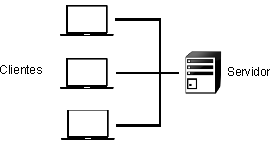
\includegraphics[width=0.75\mycolumnwidth]{Cliente_servidor/Servidores_y_clientes.pdf}
\caption{\small Relación entre clientes y servidores.}
\label{Fig:Servidores_y_clientes} 
\end{figure}

En el sistema cliente--servidor se presentan las siguientes características principales:

\begin{itemize}
	\item \textbf{El servidor brinda servicio a múltiples clientes}. Los clientes, por su parte, también pueden acceder a servicios en varios servidores, aunque esa multiplicidad es mucho más relevante en el caso del servidor. Piénsese, por ejemplo, en un navegador Web con el que podemos acceder a varias páginas y un servidor de una de dichas páginas. Mientras que en el cliente no accedemos simultáneamente a un gran número de páginas (si la pagina es estática solo usamos el servicio al cargarla, y no cargamos más de una capa en un instante dado), el servidor debe estar preparado para responder a muchas peticiones simultaneas y satisfacer la demanda de muchos clientes en un instante concreto.
	\item \textbf{Los clientes no dependen de la ubicación física del usuario}, el sistema operativo o la arquitectura física de la máquina. Esto es así porque el cliente no necesita conocer la lógica interna del servidor para usar sus servicios. Lo único necesario es que el servidor pueda exponer una interfaz externa que actúe como un modo de comunicación para recibir las peticiones del cliente, siendo esta comunicación siempre transparente para este último. 
	\item \textbf{La carga de proceso se puede repartir entre cliente y servidor}. En función del servicio y de las capacidades del cliente, el trabajo puede dividirse de una u otra forma entre las partes implicadas.
\end{itemize}

\index{Cliente}\index{Servidor}\index{Carga de proceso}


\subsection{Servidores}
\label{Servidores}
\index{Servidor}

El servidor es el elemento encargado de ofrecer el servicio como tal, respondiendo a las peticiones del cliente. A medida que los clientes se hacen más complejos y presentan mayor número de funcionalidades, también los servidores deben ser capaces de proporcionar servicios más elaborados. Las capacidades fundamentales a las que responden los servidores dentro del ámbito SIG pueden dividirse en los siguientes grupos:

\begin{itemize}
\item \textbf{Servir representaciones de los datos}. Los servicios de cartografía Web, tanto en sus orígenes como en la actualidad, son eminentemente gráficos, y en última instancia lo que la aplicación Web correspondiente va a hacer es mostrarnos algún tipo de imagen con un mapa formado a partir de una serie de datos geográficos. El servidor puede responder directamente a este tipo de necesidades, preparando una imagen a partir de los datos geográficos de los que dispone. En el caso de que estos sean ya imágenes ---por ejemplo, imágenes de satélite u ortofotos---, bastará servir estas, transmitiendo una versión escalada de las dimensiones exactas que el cliente necesite para representar en pantalla. En caso de que los datos sean de tipo vectorial, o bien ráster sin una forma de representación implícita ---por ejemplo, un Modelo Digital del Terreno--- es necesario emplear algún método para asignarles dicha representación. Este puede ser asignado por defecto por el servidor, que establecerá una simbología fija, o bien ofrecer un servicio más complejo en el que el cliente no solo pide una representación gráfica de una serie de datos para una zona dada, sino que además puede especificar \emph{cómo} crear esa representación.\index{Modelo Digital del Terreno}\index{Ortofotografía}

Asimismo, el servidor puede ofrecer la posibilidad de seleccionar los datos empleados para crear la representación gráfica. En términos de un SIG de escritorio esto es equivalente a seleccionar qué capas se van a representar de entre el total de las que se encuentran abiertas o bien en nuestro catálogo de datos al que tenemos acceso desde el SIG. En el caso de un servicio Web, el servidor dispone de una serie de capas a las que puede acceder, y a la hora de servir una imagen puede preparar esta usando unas u otras según las necesidades que el cliente especifique a la hora de hacer la petición del servicio. De igual modo, el orden en que se desea que las capas se pinten en el mapa también debe poder ser especificado por el cliente.

\item \textbf{Servir los datos directamente}. Una opción más flexible que lo anterior es que el servidor provea directamente los datos geográficos y sea después el cliente quien los utilice como corresponda, bien sea simplemente representándolos ---en cuyo caso debería ser el propio cliente quien establezca la simbología, ya que esta tarea ya no queda en manos del servidor--- o bien trabajando con ellos de cualquier otra forma, como por ejemplo analizándolos. 

Aunque las posibilidades son mayores en este caso, se requieren por parte del cliente unas capacidades mayores, ya que mientras que representar una imagen es algo sumamente sencillo desde el punto de vista técnico, crear esta a partir de los datos geográficos es más complejo.

\item \textbf{Servir consultas}. Un paso más allá en la funcionalidad que puede ofrecer el servidor es responder a \emph{preguntas} realizadas por el cliente relativas a los datos, ya sean estas relativas a la parte espacial de dichos datos, o bien a su componente temática. El servidor puede ofrecer como respuesta conjuntos reducidos de los datos de los que dispone, o valores que describan a estos. Estas consultas pueden ser útiles, por ejemplo, para establecer filtros previos cuando se dispone de un conjunto amplio de orígenes de datos. Un cliente Web puede obtener datos de distintos servidores, y puede consultar si, para un zona dada, estos servidores disponen de información, sin más que consultar la extensión cubierta por los datos de cada uno de ellos y comprobar si se interseca con la región de interés. En función de la respuesta, puede o no realizarse posteriormente el acceso a los datos en sí. Como veremos en el capítulo \ref{Metadatos}, los \emph{metadatos} son de gran utilidad para conseguir que este tipo de consultas se realicen de forma eficiente.\index{Metadatos}\index{Consultas}

\item \textbf{Servir procesos}. Por último, un servidor puede ofrecer nuevos datos, espaciales o no espaciales, resultantes de algún tipo de proceso o cálculo a partir de datos espaciales. En este caso, el proceso constituye en sí el servicio ofrecido por el servidor, y el cliente debe definir los parámetros de entrada de este y los posibles parámetros de ajuste que resulten necesarios. Los datos con los que se trabaja pueden ser proporcionados por el cliente, incorporándolos a su propia petición, o bien pueden residir en el propio servidor. En este último caso, el servidor ofrece tanto los datos, como la posibilidad de extraer resultados a partir de ellos, es decir, los datos y una herramienta para explotarlos. También pueden emplearse datos en un servidor distinto, a los que el servidor de procesos puede acceder si estos están disponibles, convirtiéndose en cliente de ese segundo servidor (Figura \ref{Fig:Datos_y_procesos_remotos}).

Las posibilidades que estos servicios brindan son muy numerosas. Por una parte, pueden añadirse funcionalidades avanzadas a interfaces Web, llevando a estas las capacidades propias de los SIG de escritorio. Por otra, la difusión de algoritmos de análisis geográfico resulta más sencilla, pudiendo ofrecerse estos a todo tipo de usuarios sin necesidad de ningún software especializado. Y por último, en ciertos casos pueden rebajarse los tiempos de proceso, ya que, en el caso de operaciones complejas, la mayor potencia del servidor respecto al cliente puede resultar en un mayor rendimiento. El reparto de tareas entre varios servidores (computación distribuida) es otra de las posibilidades que pueden a su vez ampliar la eficiencia de los procesos.\index{Computación distribuida}

\begin{figure}[!hbt]   
\centering
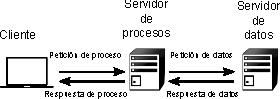
\includegraphics[width=0.75\textwidth]{Cliente_servidor/Datos_y_procesos_remotos.pdf}
\caption{\small Esquema de acceso a un servicio de procesos remotos, el cual a su vez utiliza datos de un segundo servidor. El encadenamiento de procesos permite ampliar notablemente la utilidad de estos.}
\label{Fig:Datos_y_procesos_remotos} 
\end{figure}

\end{itemize}

\subsection{Clientes}

\index{Cliente}
El cliente es el elemento que utiliza los datos proporcionados por el servicio. Para ello, realiza una petición a la que el servicio responde enviando dichos datos, que serán los que después se emplearán para realizar cualquier otra tarea, principalmente la representación de estos para que el usuario pueda visualizarlos. El cliente es, de este modo, el intermediario entre el usuario y los servicios y datos que el servidor ofrece.

Como hemos visto al estudiar los servidores, las principales capacidades de estos implican la transmisión de imágenes con cartografía ya elaborada, o bien directamente capas, ya sean de tipo ráster o vectoriales. En algunos casos, el servicio ofrecido es un servicio de procesos, pero su resultado generalmente es también una capa, por lo que, desde el punto de vista del cliente, la funcionalidad es en cierto modo similar (aunque internamente requiera una implementación por completo distinta).

El cliente, por tanto, debe disponer de capacidades para formular peticiones a servidores como los anteriormente descritos, así como para emplear las posibles respuestas que estos devolverán. Estas últimas incluyen por lo general componentes de representación, habitualmente con la forma típica de un visor en el que se permite cambiar la escala y desplazar la vista, tal y como ya vimos en el capítulo \ref{SIGs_escritorio}. No obstante, estas capacidades pueden variar ampliamente de un cliente a otro, desde el mínimo necesario para simplemente representar los datos obtenidos del servidor hasta conjuntos de funcionalidades mucho más avanzadas pensadas para un uso intensivo de esos mismos datos.

Distinguimos así dos tipos de clientes en función de las capacidades que tengan: \emph{clientes ligeros} y \emph{clientes pesados}.

\begin{itemize}
	\item \textbf{Cliente ligero}. Se denomina \emph{ligero} por el tamaño relativamente reducido del programa en sí, lo cual va consecuentemente asociado a unas capacidades limitadas. Hablamos de clientes ligeros cuando nos referimos a \emph{Web Mapping} y a clientes que se ejecutan sobre un navegador Web, los cuales son siempre sencillos en cuanto a sus funcionalidades. En el momento de la carga de la página Web que contiene al cliente, el navegador descarga toda la lógica del programa, lo cual hace necesario limitar el tamaño de este.
	
	No obstante, los clientes Web empiezan progresivamente a ampliar sus posibilidades, y en ello juegan un importante papel otros servicios distintos a los de mapas o los de datos, como pueden ser los de procesos. Estos permiten que las funcionalidades adicionales no se implementen en el propio cliente (y por tanto sin aumentar en exceso su tamaño y sin disminuir su <<ligereza>>), sino que sean accedidas también como servicios remotos.
	
	La evolución de la cartografía Web en esta dirección se dirige desde el \emph{Web Mapping} al \emph{Web GIS}, tal y como comentamos algunas páginas atrás.
	
	\item \textbf{Cliente pesado}. A diferencia del cliente ligero, el cliente \emph{pesado} es una aplicación individual que no se ejecuta sobre otra aplicación soporte como puede ser un navegador Web. Al ser un programa independiente, debe ocuparse de toda la lógica del proceso y de proveer todas las funcionalidades necesarias, por lo que su tamaño es generalmente mayor. Pese a ello, un cliente pesado no ha de ser necesariamente más potente y con más funcionalidades que uno ligero (aunque habitualmente lo es), ya que existen aplicaciones muy sencillas con capacidad para conectarse a servicios de mapas, que ofrecen poco más que un visor de cartografía. La diferencia no estriba en las capacidades del programa, sino en el enfoque a la hora de implementar este y el uso o no de otra aplicación <<plataforma>>, generalmente en forma de un navegador Web.
	
	Los clientes pesados suelen permitir el uso de datos no procedentes directamente del acceso a servicios, tales como datos en ficheros locales, y no están pensados exclusivamente como clientes, sino como aplicaciones más amplias que además disponen de capacidades para aprovechar un determinado tipo de servicios. Dicho de otro modo, un cliente pesado tal y como un SIG de escritorio tiene utilidad aunque no se emplee como cliente de ningún servicio y no se disponga de conexión a red alguna, ya que puede alimentarse con datos locales y todas sus restantes funcionalidades (análisis, preparación de cartografía, etc.) pueden aprovecharse con dichos datos.
\end{itemize}

\index{Cliente!ligero}\index{Cliente!pesado}

\section{Limitaciones y problemas de la cartografía Web}

Trasladar las ideas de los SIG de escritorio a la Web no es sencillo, por cuanto el entorno en el que nos movemos es muy distinto en uno y otro caso. La Web tiene sus propias limitaciones e inconvenientes, que en muchos casos no existen en el caso de una aplicación de escritorio, y este hecho presenta dificultades complejas de salvar, obligando a desarrollar soluciones alternativas.

Una limitación básica es la impuesta por el propio navegador como marco de trabajo. Las propias ventajas que este aporta son también responsables de ciertas limitaciones, ya que en el desarrollo de una aplicación SIG Web no se tiene la misma libertad que al desarrollar una aplicación de escritorio. Este no es un problema exclusivo del \emph{Web Mapping}, sino en general de todas las aplicaciones Web, que, pese a los avances que han tenido lugar en este sentido y la rápido evolución de las tecnologías Web, siguen sin poder ofrecer exactamente las mismas funcionalidades en lo que a interfaces respecta. 


A lo anterior debemos sumar el hecho de que las tecnologías Web en general son recientes y en cierto modo inmaduras, y aunque se emplea gran cantidad de medios y esfuerzo en el ámbito Web debido a su vital importancia en la actualidad, una buena parte de los elementos tecnológicos sobre los que se fundamenta el \emph{Web Mapping} actual no están todavía completamente desarrollados y necesitan aún evolucionar.

El aspecto más problemático es, no obstante, la propia red, especialmente en lo que respecta a su fiabilidad y rendimiento. Todos los datos que el cliente emplea en una aplicación de cartografía Web provienen de la red, y por tanto existe una fuerte dependencia entre la aplicación y el funcionamiento tanto de esta como del servidor que a través de ella nos proporciona esos datos.

Si abrimos un archivo con datos espaciales en nuestro ordenador desde un SIG de escritorio, podemos casi garantizar que esa misma operación funcionará de igual modo si la repetimos en otro momento. Tener esa misma seguridad cuando se trabaja con datos remotos no es tan sencillo, ya que la red puede no funcionar o el servidor puede estar recibiendo en este momento gran cantidad de peticiones de otros clientes y no ser capaz de gestionarlas eficientemente y ofrecernos al instante respuesta a nuestra petición. En definitiva, las mismas circunstancias que afectan a todas las aplicaciones Web y que son conocidas por todos.

El rendimiento de la red es más importante aún si cabe en el caso de trabajar con información geográfica, ya que los datos suelen ser voluminosos. Visualizar un mapa y que este pueda desplazarse y modificarse de forma igual de fluida que al trabajar con una aplicación de escritorio requiere por un lado un ancho de banda suficiente para transmitir la gran cantidad de datos necesarios, y por otro la implementación de algunas técnicas particulares que facilitan este proceso. Por su importancia, veremos en detalle las técnicas de \emph{tiling} (división horizontal de los datos geográficos en teselas) y \emph{cacheo} (almacenamiento temporal de datos en la máquina del cliente), utilizadas habitualmente en la actualidad.

\subsection{\emph{Tiling} y \emph{cacheo}}

\index{Tiling}\index{Cacheo}

Dos técnicas básicas que se emplean actualmente en los clientes Web que manejan información geográfica son el \emph{tiling} y el \emph{cacheo}. Estas técnicas permiten que la experiencia de trabajar con información geográfica dentro de una aplicación SIG Web sea más agradable, logrando una mayor fluidez y superando en cierta medida las limitaciones de la red. Aunque es cierto que cada vez disfrutamos de mayores anchos de banda y velocidades de transmisión más altas, también aumentan de igual modo los volúmenes de datos manejados, con lo que las dificultades siguen existiendo de manera similar.

Ambas técnicas se utilizan en servicios en los que el servidor provee imágenes, ya que es en estos en los que resultan aplicables, y también donde es más necesario recurrir a este tipo de técnicas.

El \emph{tiling} es una técnica consistente en dividir las imágenes con las que se trabaja en imágenes menores que formen un mosaico. Esto permite un trabajo más rápido, al utilizar unidades mínimas de menor tamaño y poder reducir la necesidad de transmitir datos a través de la red si se realiza una gestión correcta del conjunto de elementos de ese mosaico.

Esta división es similar en forma a la propia que se da en los datos originales, ya que, como sabemos (véase sección \ref{divisionHorizontal}), estos también se encuentran divididos horizontalmente. No obstante, se trata de una estrategia propia del sistema cliente--servidor, que divide las propias imágenes que luego se representarán en este último, de forma que en lugar de transmitir una única imagen se transmiten varias de menor tamaño y la información correspondiente a la posición relativa de estas.

El \emph{cacheo}, por su parte, es una técnica no exclusiva del ámbito SIG, sino de la Web en general, y consiste en almacenar de forma temporal los datos obtenidos de un servidor en la máquina local o bien en una máquina intermedia (\emph{proxy}\index{Proxy}). De este modo, si volviera a resultar necesario acceder a esos datos, no han de pedirse al servidor, sino que pueden recuperarse de la copia local, con las ventajas que ello tiene en cuanto a la velocidad de acceso y la fiabilidad del proceso.

El uso conjunto de \emph{tiling} y \emph{cacheo} puede disminuir sensiblemente el volumen de datos a transmitir para, por ejemplo, modificar el encuadre de un mapa en una aplicación SIG Web. La figura \ref{Fig:Tiling} muestra un ejemplo sencillo que servirá para comprender el ahorro de datos que puede conseguirse con el uso conjunto de estas técnicas.

\begin{figure}[!hbt]   
\centering
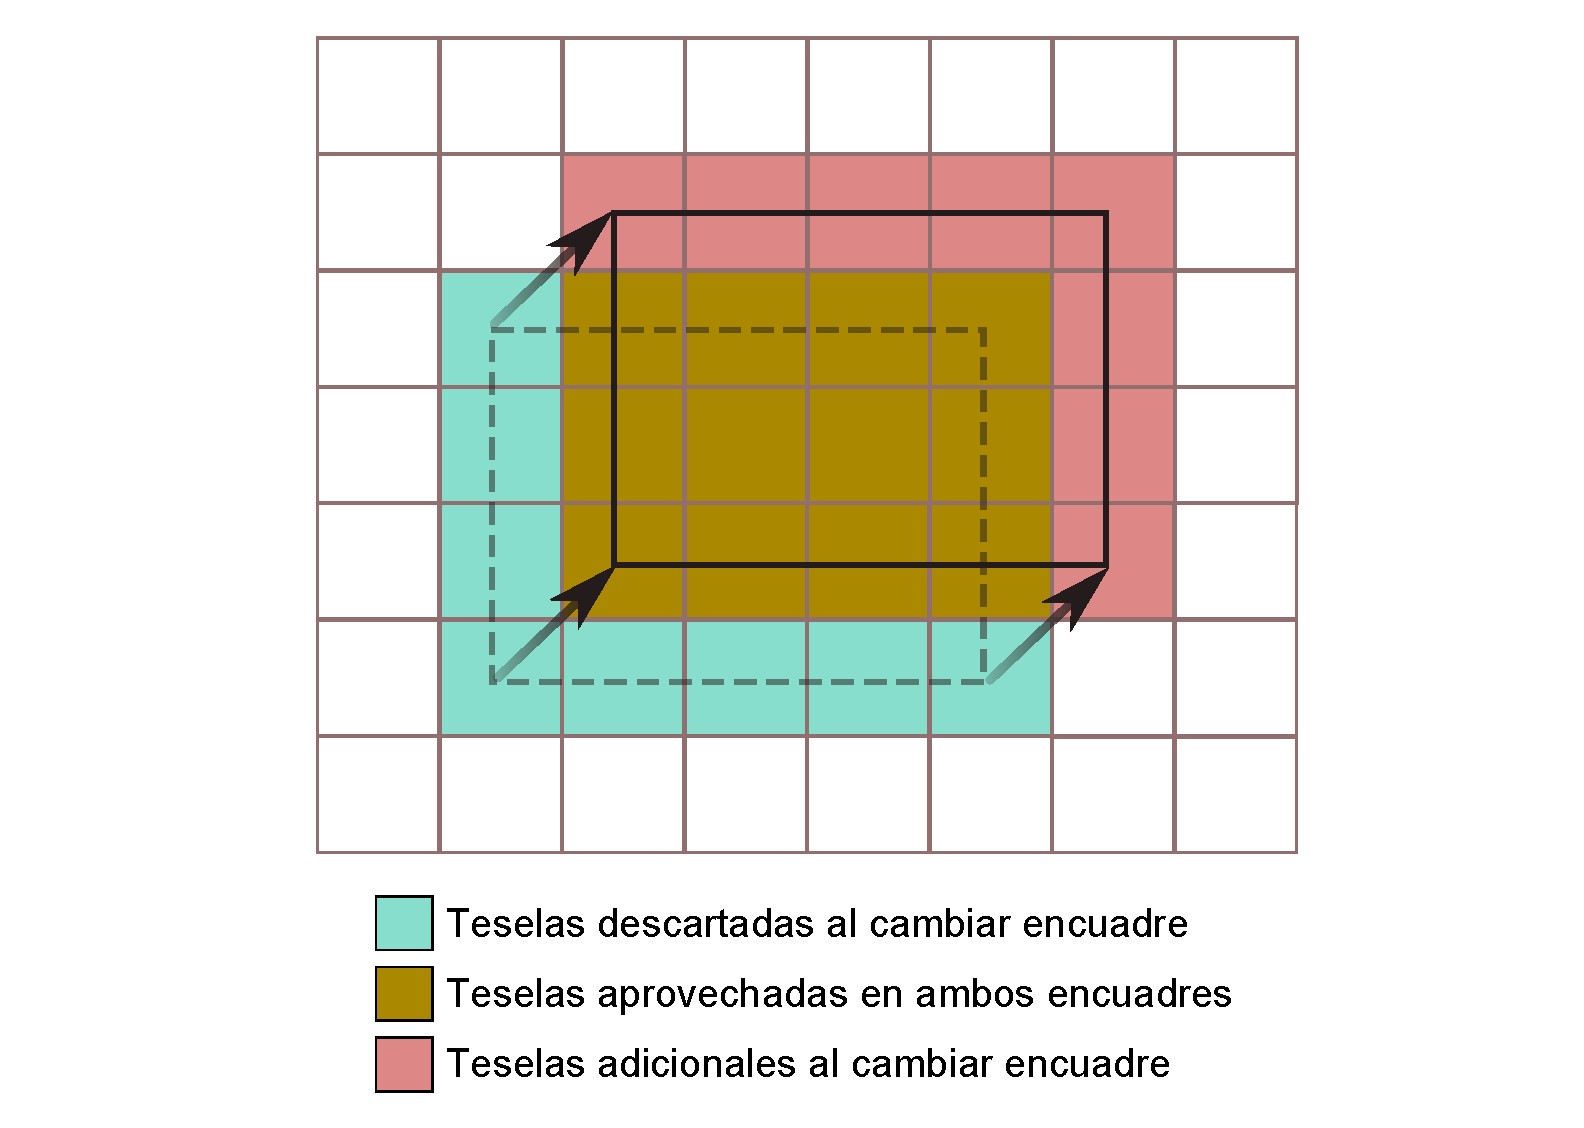
\includegraphics[width=.8\textwidth]{Cliente_servidor/Tiling.pdf}
\caption{\small Esquema del uso de \emph{tiling} y \emph{cacheo} para optimizar la transmisión de datos en una aplicación SIG Web}
\label{Fig:Tiling} 
\end{figure}

En la figura puede verse del dato global al que se accede, dividido en una serie de unidades. Ello no quiere decir que el dato tenga ese número de divisiones o que existan otros tantos ficheros. Puede tratarse de un único fichero, o de un número muy elevado de ellos. Las divisiones se realizan a efectos de crear el mosaico de imágenes a la hora de transmitir estas.

Inicialmente, la aplicación Web encuadra una región que cubre 20 elementos o teselas. Si el usuario desplaza el encuadre para que cubra otro área distinta, como en el caso mostrado en la figura, el cliente realizará una nueva petición y obtendrá una nueva imagen, que tendrá exactamente el tamaño con que esa imagen va a representarse. Este es exactamente el mismo tamaño que la imagen que encontramos inicialmente en el encuadre original, y por tanto la representación de este encuadre original y posteriormente el encuadre modificado requiere transmitir dos imágenes que cubren cada una de ellas veinte teselas.

Si, por el contrario, aplicamos conjuntamente las técnicas anteriores de \emph{tiling} y \emph{cacheo}, al variar el encuadre no es necesario obtener del servidor una imagen que cubra todo el área a representar, sino tan solo los 8 elementos correspondientes a la zona no cubierta por la imagen inicial, ya que los restantes ya habrán sido obtenidos con anterioridad y se encontrarán almacenados (\emph{cacheados}) en nuestro ordenador. Es decir, el cliente crea la imagen a representar con 8 subimagenes pedidas al servidor y otras 12 ya descargadas previamente, reduciendo sensiblemente el volumen de datos pedidos al servidor.

Cuando este esquema de funcionamiento se combina con tecnologías como AJAX, citada anteriormente, y que añade a su vez mayor fluidez y una mejor respuesta de la aplicación Web, el resultado es una aplicación SIG altamente funcional y cuyo comportamiento se asemeja en cuanto a rendimiento al de un SIG de escritorio trabajando con datos locales.\index{AJAX}

Este tipo de técnicas no son exclusivas de los SIG en Internet, sino que también se aplican por igual al caso de SIG de escritorio cuando estos actúan como clientes y acceden a datos remotos. Particularmente, son de especial relevancia en el caso de los globos tridimensionales, en los cuales estas mismas técnicas se aplican no solo para las imágenes a visualizar, sino también para los datos de elevación empleados para dar forma al relieve.

La combinación de \emph{tiling} y \emph{cacheo} se lleva a cabo a múltiples escalas, de forma que se reduce el número de operaciones a realizar y se obtiene un mayor rendimiento. Se emplean las denominadas \emph{pirámides}, que ya vimos en el apartado \ref{Generalizacion_en_SIG} dedicado a la generalización cartográfica en un SIG. Estas pueden ser empleadas también en el lado del servidor, incluso cuando este sirve mapas creados a partir de cartografía vectorial. Para evitar tener que rasterizar los datos vectoriales cada vez que se realiza una petición (lo cual supondría un gran coste en términos de proceso), se rasterizan de antemano a distintas escalas, de forma que cuando el cliente efectúa la petición ya se dispone de una imagen que servirle, sea cual sea la escala que pida.\index{Pirámides}.

Una técnica de reciente aparición es la denominada emph{tiling vectorial}. Aplicando los mismos principios que el \emph{tiling}, es decir, la subdivision de los datos de forma regular, las capas vectoriales se <<trocean>> en el origen y se envían después solamente los datos necesarios para el area cubierta en el cliente. Combinando este enfoque con el uso de capas con distinto detalle según la escala, se logran dos ventajas: 

\begin{itemize}
\item Disminución del volumen de datos. 
\item Capacidad de modificar la simbología en el cliente.
\end{itemize}

Al enviar los datos en lugar de una representación de estos, el cliente es quien debe establecer la simbología, lo cual permite que sea el usuario quien seleccione cómo representar los elementos vectoriales. Al mismo tiempo, se logran ventajas en la experiencia de usuario, debidas principalmente a la escalabilidad de los datos vectoriales, que permite por ejemplo presentar transiciones más fluidas cuando se modifica la escala del mapa.

Obviamente, este tipo de enfoque es válido unicamente para el caso de capas vectoriales.

\section{Resumen}

Hemos visto en este capítulo las ideas fundamentales del binomio cliente--servidor, tanto en su definición más general referente a servicios Web de cualquier tipo, como en aquellos específicos del ámbito SIG. En base a esto, existen distintas formas de llevar a la red tanto los propios datos geográficos como las funcionalidades principales de los SIG de escritorio, y que pueden variar en cuanto a su complejidad, desde simples mapas estáticos hasta aplicaciones Web complejas. Pese a las elevadas posibilidades que existen hoy en día en cuanto a tecnologías Web, es importante conocer también las limitaciones del entorno de trabajo, las cuales derivan tanto de la propia red como de otros aspectos, por ejemplo el hecho de que la aplicación Web se ejecute dentro de un navegador. Estas limitaciones llevan al desarrollo de técnicas particulares para optimizar el funcionamiento de las aplicaciones SIG Web, entre las que se han de destacar el \emph{tiling} y el \emph{cacheo}.

Asimismo, conocemos ya las funcionalidades principales que debe presentar un servidor para responder a las peticiones de un cliente SIG, que son principalmente servir representaciones de los datos geográficos, servir los datos en sí o consultas sobre estos, o bien servir procesos de análisis basados en dichos datos.

\pagestyle{empty}